% !TeX program = xelatex
\documentclass[12pt,a4paper,oneside]{report}

\usepackage{fontspec}
\setmainfont{DejaVu Serif}
\setsansfont{DejaVu Sans}
\setmonofont{DejaVu Sans Mono}
\usepackage[a4paper,top=2.5cm,bottom=2.5cm,left=3.2cm,right=2.3cm]{geometry}
\usepackage{amsmath,amssymb,mathtools}
\usepackage{booktabs,longtable,tabularx,array,multirow}
\usepackage{graphicx,float}
\usepackage{xcolor}
\usepackage{enumitem}
\usepackage{caption}
\usepackage{subcaption}
\usepackage{fancyhdr}
\usepackage{microtype}
\usepackage{setspace}
\usepackage{url}
\usepackage[hidelinks,unicode]{hyperref}

\graphicspath{{figures/}}
\definecolor{darkred}{RGB}{150,35,35}
\setstretch{1.35}
\setlength{\parindent}{1.2cm}
\setlength{\parskip}{0.25em}
\setlength{\emergencystretch}{3em}
\setlist[itemize]{topsep=0.3em,itemsep=0.2em}
\setlist[enumerate]{topsep=0.3em,itemsep=0.2em}
\renewcommand{\arraystretch}{1.18}

\pagestyle{fancy}
\fancyhf{}
\fancyhead[L]{\small RNA 3D thesis}
\fancyhead[R]{\small TBM, DRfold2, and geometry refinement}
\fancyfoot[C]{\thepage}
\setlength{\headheight}{15pt}

\hypersetup{
  pdftitle={A Hybrid Template-Based and Deep-Learning Framework for RNA Three-Dimensional Structure Prediction},
  pdfauthor={Do Thanh Dat},
  pdfsubject={Master thesis draft},
  pdfkeywords={RNA 3D, TBM, DRfold2, temporal leakage, geometry refinement, TM-score}
}

\newcommand{\cprime}{C1$^{\prime}$}
\newcommand{\angstrom}{\text{\AA}}
\newcommand{\todo}[1]{\textcolor{darkred}{\textbf{[TO COMPLETE: #1]}}}
\newcommand{\T}{\mathrm{T}}
\newcommand{\D}{\mathrm{D}}

\begin{document}

\begin{titlepage}
\begin{center}
  {\large UNIVERSITY OF SCIENCE AND TECHNOLOGY OF HANOI}\\[0.25cm]
  {\large ICT LAB}\\[1.6cm]
  {\Large\bfseries DO THANH DAT}\\[1.5cm]
  {\Large\bfseries
  A HYBRID TEMPLATE-BASED AND DEEP-LEARNING\\
  FRAMEWORK FOR RNA THREE-DIMENSIONAL\\
  STRUCTURE PREDICTION WITH\\
  TEMPORAL LEAKAGE CONTROL AND\\
  GEOMETRY REFINEMENT
  }\\[1.5cm]
  {\large MASTER THESIS}\\[0.5cm]
  {\large DATA SCIENCE}\\[1.6cm]
  \begin{tabularx}{0.94\textwidth}{lX}
  Supervisors: & NGUYEN MINH HUONG\\
  & NGUYEN CAM LINH\\
  Student ID: & 2440059
  \end{tabularx}
  \vfill
  {\large HANOI, 2026}
\end{center}
\end{titlepage}

\pagenumbering{roman}

\chapter*{Declaration}
\addcontentsline{toc}{chapter}{Declaration}
\todo{Insert the declaration required by the university template.}

\chapter*{Acknowledgements}
\addcontentsline{toc}{chapter}{Acknowledgements}
\todo{Acknowledge supervisors, the degree program, colleagues, and family.}

\chapter*{Abstract}
\addcontentsline{toc}{chapter}{Abstract}

Predicting the three-dimensional structure of RNA from sequence remains difficult
because the conformational space is large, experimental structures are limited, and RNA
is intrinsically flexible \cite{zhang_experimental_review,rna_progress_review,
state_of_rnart}. This thesis develops a hybrid pipeline that combines time-safe
template-based modeling, DRfold2 as an independent candidate source, and geometry
refinement for local correction. The system produces three template-derived structures
and two DRfold2 structures, then refines each candidate without access to native labels.
This design matches the best-of-five evaluation used in the Stanford RNA 3D Folding
competition \cite{competition_paper,kaggle_competition}.

The evidence is separated into local component studies and external hidden-set
evaluation. The local protocol uses 60 temporally earlier RNAs to estimate geometric
priors, 20 RNAs to select the configuration, and 20 family-disjoint newer RNAs for a
single confirmatory evaluation. In the TBM component study, MMseqs2 returned a template
for 8 of 20 calibration targets, whereas composite search produced candidates for all
20. The composite score therefore increased retrieval coverage, although its full
weighted form did not clearly outperform global alignment alone.

On the 20 held-out RNAs, the best available score from three TBM candidates averaged
0.565183, and the corresponding score from two DRfold2 candidates averaged 0.502627.
Their union reached 0.588304, a gain of 0.023121 with a target-bootstrap 95\% confidence
interval of $[0.006444,0.047519]$. DRfold2 supplied the better source on 8 of 20 targets,
indicating complementarity rather than higher average accuracy. Geometry refinement
increased \cprime{}-lDDT by 0.006660 and reduced SW-RMSD9 by 0.040386~\angstrom{}, while
TM-score changed by $-0.001107$ with a confidence interval that included zero. The
refinement therefore corrected local relationships while approximately preserving the
global fold.

On Kaggle, the time-safe TBM pipeline scored 0.60084 on the public set and 0.60175 on the
private set. The final three-TBM, two-DRfold2 pipeline with geometry refinement reached
0.62809 and 0.61390, respectively, exceeding the reported 0.59298 private score of the
reference TBM-only notebook. Because the final submission changed both candidate
composition and refinement, this difference is interpreted at the pipeline level.
Together with the local factorial experiment, the results support candidate-source
complementarity as the primary mechanism for global TM improvement, while geometry
refinement provides a separate benefit in local trace quality.

\noindent\textbf{Keywords:} RNA three-dimensional structure, template-based modeling,
DRfold2, TM-score, \cprime{}-lDDT, temporal safety, geometry refinement.

\tableofcontents
\listoftables
\listoffigures
\clearpage
\pagenumbering{arabic}

\chapter{Introduction}
\label{chap:intro_en}

\section{Background and motivation}

RNA regulates gene expression, catalyzes reactions, recognizes molecular partners, and
forms ribonucleoprotein complexes. These functions depend not only on the order of A, C,
G, and U, but also on the base pairs, motifs, and three-dimensional arrangements formed
by the chain \cite{cao_rna_functions,tinoco_folding,butcher_tertiary}. Secondary
structure describes base pairing and local motifs, whereas tertiary structure captures
how these elements interact in space \cite{tinoco_folding,butcher_tertiary}. An RNA 3D
predictor must consequently recover both the global fold and its local geometry.

X-ray crystallography, nuclear magnetic resonance, and cryogenic electron microscopy
are major routes to experimental RNA structures. Each technique has a distinct domain
of applicability, and cryo-EM has expanded access to large RNA-containing complexes;
nevertheless, sample preparation, data acquisition, and model reconstruction remain
resource-intensive \cite{zhang_experimental_review,ma_cryoem}. The PDB provides the
global archive for experimentally determined macromolecular structures, but RNA remains
less represented than protein and many RNA families lack close structural templates
\cite{pdb_archive,zhang_experimental_review}. This gap motivates computational
prediction from sequence.

Current RNA 3D methods draw on physical principles, knowledge extracted from observed
structures, and learned patterns. Template-based modeling can be highly accurate when a
suitable structural relative is recognized, whereas deep models can produce candidates
when direct template retrieval is weak \cite{rna_progress_review,drfold,rhofoldplus,
drfold2}. Blind RNA-Puzzles and CASP assessments show that rankings vary across targets,
lengths, fold novelty, and permitted information \cite{rna_puzzles,casp15,
state_of_rnart}. A bank of candidates from different sources is therefore attractive
when the evaluation retains the best of several predictions.

The Stanford RNA 3D Folding competition provides a particularly relevant setting. More
than 1,700 teams predicted 43 previously unreleased structures, and both leading systems
used TBM. Post-competition analysis further showed that combining TBM and deep learning
could outperform individual components on the same test set \cite{competition_paper}.
This observation does not make every RNA a template-rich problem. Instead, it motivates
two questions: how to retrieve structures without future information, and how to cover
targets for which templates are inadequate.

\section{Research problem}

A TBM pipeline can receive an artificially high score if its library contains a
structure released after the prediction cutoff. This temporal leakage uses information
that is public at rerun time but unavailable in the original blind setting. RNA-Puzzles
and CASP explicitly separate prediction from unreleased structures, making the data
cutoff part of the scientific protocol \cite{rna_puzzles,casp15,competition_paper}.
This thesis requires every template to predate its target and excludes the target's own
reference PDB entries.

Even under a valid cutoff, a single retrieval system may miss useful templates. MMseqs2
supports fast, sensitive sequence search at database scale \cite{mmseqs2}, but structural
relatives do not always present a sufficiently strong homolog for the fast retrieval
path. We therefore complement MMseqs2 with a search heuristic based on global alignment,
local alignment, sequence composition, and 3-mer overlap. Its purpose is to increase
candidate recall rather than define an optimal biological score.

TBM cannot provide a strong model for every target. DRfold2 is therefore introduced as
an independent source rather than a replacement for templates. DRfold2 extends the line
of work that combines end-to-end learning with learned geometric potentials for RNA 3D
prediction \cite{drfold,drfold2}. Retaining three TBM and two DRfold2 models preserves
template strength on easier targets while reserving two slots for folds that the deep
model may recover better.

Candidates from both branches may still contain irregular backbone distances, clashes,
or local distortions. Previous nucleic-acid refinement tools show that better geometric
quality does not guarantee systematic improvement in native RMSD \cite{qrnas,arena}.
The refinement objective in this thesis is therefore narrow: improve local \cprime{}
geometry while keeping TM-score within a predeclared preservation margin. Refinement is
not presented as a second global-fold predictor.

\section{Research questions}

The thesis addresses three questions in the order in which information enters the
pipeline:

\begin{description}[leftmargin=1.4cm,style=nextline]
  \item[RQ1.] What does composite search add to MMseqs2 in a time-safe TBM pipeline, and
  which ranking components produce measurable changes?
  \item[RQ2.] When candidate count is controlled, does DRfold2 complement the targets
  missed by TBM?
  \item[RQ3.] Does geometry refinement improve \cprime{}-lDDT and sliding-window RMSD
  while preserving global TM-score?
\end{description}

These questions form a testable progression. RQ1 explains candidate availability, RQ2
tests source diversity, and RQ3 identifies the structural scale affected by postprocessing.
The leaderboard is used as an external assessment of the frozen pipeline, not as a
substitute for local ablation.

\section{Contributions}

The first contribution is an auditable time-safe TBM branch that unifies fast and
composite retrieval, enforces release-date and self-PDB filters, realigns candidates,
ranks them by identity and coverage, and transfers \cprime{} coordinates. Component
studies evaluate each decision instead of inferring its value from a single final score.

The second contribution is quantitative evidence of complementarity between TBM and
DRfold2. The study reports each source, their union, and fixed-size candidate banks.
Fixed-N comparisons partially separate genuine source effects from the mechanical
benefit of adding more prediction slots.

The third contribution is conservative geometry refinement evaluated with a held-out
protocol. Priors are estimated on 60 RNAs, the configuration is selected on 20, and the
method is frozen before opening 20 newer RNAs. Raw candidates, a simple smoothing
baseline, the full objective, cumulative ablation, and leave-one-out ablation are all
reported.

Finally, the thesis provides a two-level explanation of leaderboard performance. The
0.61390 private score establishes external pipeline value, while local complementarity
and refinement experiments identify component-level mechanisms. Keeping these evidence
levels separate prevents the refinement stage from receiving unsupported credit for the
entire score increase.

\section{Scope and organization}

The system predicts one \cprime{} coordinate per nucleotide and returns five structures
per target. Confirmatory local analysis covers single-chain RNAs up to 96 nucleotides;
Kaggle provides an external check on a different distribution that includes longer
targets. Full-atom chemistry, ions, ligands, chemical modifications, and RNA-protein
interfaces are outside the evaluated representation, although each can be important to
RNA structure and function \cite{butcher_tertiary,zhang_experimental_review}.

Chapter~\ref{chap:background_en} reviews the scientific and computational background.
Chapter~\ref{chap:data_en} describes the data and leakage controls.
Chapter~\ref{chap:method_en} presents the pipeline, and
Chapter~\ref{chap:experiment_en} defines the experiments. Results are reported in
Chapter~\ref{chap:results_en}, followed by discussion in
Chapter~\ref{chap:discussion_en} and conclusions in Chapter~\ref{chap:conclusion_en}.

\chapter{Background and Related Work}
\label{chap:background_en}

\section{RNA structural organization}

RNA is a polymer with a sugar-phosphate backbone and four primary bases. Watson-Crick
interactions, base stacking, noncanonical pairs, ions, and tertiary contacts contribute
to structural stability \cite{tinoco_folding,butcher_tertiary}. Interactions that are
distant in sequence can become adjacent in space, allowing a local motif error to alter
the molecular arrangement. Local and global quality must therefore be measured with
different metrics.

This thesis uses the \cprime{} trace as a common representation. For a sequence of
length $L$, a candidate is
\begin{equation}
X=[\mathbf{x}_1,\ldots,\mathbf{x}_L]^\T\in\mathbb{R}^{L\times3},
\end{equation}
where $\mathbf{x}_i$ is the \cprime{} coordinate of nucleotide $i$. This coarse-grained
form matches the competition output \cite{competition_paper,kaggle_competition}. It
does not encode base orientation or full chemistry, so conclusions are limited to fold
and \cprime{}-trace quality.

Rigid rotation and translation do not alter internal structure. Kabsch superposition
finds the rotation that minimizes squared deviations for known correspondence
\cite{kabsch}. lDDT avoids global superposition, whereas TM-score searches for a
structural alignment and uses length-dependent normalization
\cite{tm_score,lddt,usalign}. The metrics consequently respond to distinct scales of
structural error.

\section{Template-based modeling}

TBM assumes that a known structure can provide a scaffold for a related query. A typical
workflow retrieves templates, aligns query and template, transfers corresponding
coordinates, builds unsupported regions, and refines the model
\cite{rna_progress_review,competition_paper}. Accuracy depends on both recognizing a
suitable structure and aligning residues correctly. High identity over a short fragment
may be less useful than weaker similarity over nearly the complete target.

Needleman-Wunsch solves global sequence alignment, whereas Smith-Waterman identifies the
best local alignment \cite{needleman_wunsch,smith_waterman}. The two algorithms expose
different signals: global alignment measures whole-chain agreement and local alignment
recognizes conserved regions. The composite search combines both with composition and
3-mer features to broaden retrieval.

MMseqs2 enables sensitive search over large sequence collections
\cite{mmseqs2}. Retrieval speed, however, is not equivalent to structural coverage. The
experiments therefore report availability, conditional quality when a hit exists, and
whole-cohort means separately. This prevents the 12 targets without MMseqs2 hits from
silently disappearing from the evaluation.

\section{Deep RNA structure prediction}

Recent deep models learn sequence representations, geometric distributions, or
coordinates for RNA. ARES applies geometric deep learning to structure scoring, DRfold
combines end-to-end prediction with learned potentials, RhoFold+ uses an RNA language
model, and DRfold2 develops a more efficient predictive pipeline
\cite{ares,drfold,rhofoldplus,drfold2}. Although these approaches reduce direct
dependence on a close template, their accuracy remains target and benchmark dependent
\cite{state_of_rnart,drfold2}.

DRfold2 is not framed as a universal replacement for TBM in this thesis. The sources
have distinct failure modes: TBM depends on retrieval and alignment, whereas a pretrained
model depends on its training distribution and learned evolutionary signals. A common
candidate bank exploits this difference, and the held-out experiment tests whether the
difference is useful in practice.

\section{Structure refinement}

Refinement searches the neighborhood of a candidate for structures that better satisfy
geometric or energetic constraints. QRNAS optimizes nucleic-acid models with an extended
energy function, and Arena reconstructs full-atom RNA from coarse-grained predictions
\cite{qrnas,arena}. This literature distinguishes stereochemical regularization from
movement toward the native structure. Better bonds and fewer clashes do not guarantee a
better global fold.

The refinement in this thesis follows the same distinction. A source restraint preserves
the initial candidate; distance, angle, and torsion priors regularize the trace; and
clash, kink, and radius-of-gyration terms target specific artifacts. Effectiveness is
measured primarily with TM-score, \cprime{}-lDDT, and sliding-window RMSD rather than the
optimized loss itself \cite{tm_score,lddt,usalign}.

\section{Structural evaluation}

TM-score was introduced as a length-normalized measure of structural similarity
\cite{tm_score}, and US-align extends structural alignment to nucleic acids and
macromolecular complexes \cite{usalign}. The competition scores each target using the
best combination of five predictions and available native conformations, then averages
over targets \cite{competition_paper}. In this thesis, best-of-five is an evaluation
oracle only; inference never uses native structures to select a candidate.

lDDT evaluates local distance preservation without global superposition \cite{lddt}.
We compute it on \cprime{} atoms and denote it \cprime{}-lDDT. Sliding-window RMSD
superposes each contiguous window by Kabsch and then measures coordinate deviation;
windows of 9 and 15 nucleotides respond more strongly to local distortions than a
31-residue window or whole-structure RMSD \cite{kabsch}. Together, these metrics separate
local trace correction from global fold change.

\section{Research gap}

Benchmarking studies compare RNA 3D predictors, and the competition analysis shows that
TBM remains competitive as structural databases grow
\cite{state_of_rnart,competition_paper}. A leaderboard score, however, does not reveal
which component produced the result, and a component study without a temporal cutoff
can favor template search. The first gap is therefore a white-box study of TBM under a
realistic release-date policy.

The second gap concerns source complementarity under controlled candidate count. A
five-model union can beat a three-model bank merely because it has more opportunities.
This thesis reports both union and fixed-N comparisons. The final gap is confirmatory
evaluation of geometry refinement against raw candidates, a simple baseline, independent
metrics, and ablations. These gaps map directly to the three research questions.

\chapter{Data and Evaluation Controls}
\label{chap:data_en}

\section{Data sources and splits}

The template library is built from public PDB structures. The PDB is the single global
archive for macromolecular structural data and supplies chain, sequence, coordinate, and
release metadata \cite{pdb_archive}. The frozen project snapshot contains 8,670
structure files, 23,869 RNA or RNA-DNA chains, and approximately 10.86 million residues.
About 99.9\% of residues contain a \cprime{} coordinate. The MMseqs2 index has roughly
20,844 valid chains, while the deduplicated composite library has 7,155 unique sequences.
These counts describe the project artifact rather than the current PDB.

The initial development set contains 12 CASP15 targets of 30 to 720 nucleotides. CASP is
a blind assessment in which target structures are unreleased during prediction, and its
RNA targets have an official independent assessment \cite{casp15}. Because this cohort
is small and intentionally difficult, it is used for development, leakage illustration,
and deployment checks rather than as the only confirmatory evidence.

The principal study uses 100 RNAs released between January 2024 and March 2025. Every
target has three blindly generated TBM candidates and two DRfold2 candidates. The data
are split temporally into 60 train, 20 calibration, and 20 validation RNAs as shown in
Table~\ref{tab:splits_en}. An audit found no sequence group or family group crossing a
split.

\begin{table}[H]
\centering
\caption{Data split for geometry refinement and complementarity analysis.}
\label{tab:splits_en}
\begin{tabularx}{\textwidth}{l r p{4.2cm} X}
\toprule
Split & RNAs & Release-date range & Role \\
\midrule
Train & 60 & 2024-01-10 to 2024-12-04 & Estimate geometric priors \\
Calibration & 20 & 2024-12-11 to 2025-01-08 & Select and freeze configuration \\
Validation & 20 & 2025-01-15 to 2025-03-26 & One confirmatory evaluation \\
\bottomrule
\end{tabularx}
\end{table}

The dominant feature of Table~\ref{tab:splits_en} is role separation. Train creates
statistics, calibration determines hyperparameters, and validation measures the frozen
method. No validation result is used to revise the configuration. This protocol cannot
remove every distribution bias, but it prevents the same target from selecting and
confirming the method.

Kaggle provides external evaluation with sequences and native structures hidden during
notebook execution. The competition requires five predictions per target and scores the
best using US-align on \cprime{} atoms \cite{competition_paper,kaggle_competition}. We
retain the public and private scores, execution manifest, and final CSV hash. Because
hidden native structures are unavailable, Kaggle supplies a pipeline-level scalar rather
than per-target ablation.

\begin{figure}[H]
\centering
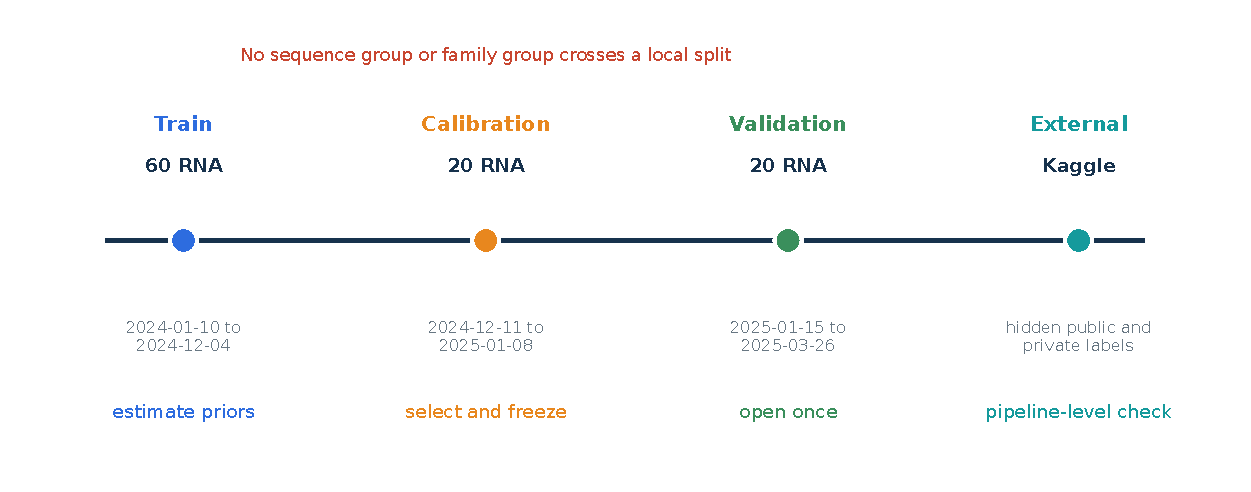
\includegraphics[width=0.96\textwidth]{evaluation_protocol.pdf}
\caption{Two-level evidence protocol. Local splits are separated by time and family;
Kaggle supplies an external hidden-set check of the complete pipeline.}
\label{fig:evaluation_protocol_en}
\end{figure}

\section{Temporal and self-template exclusion}

For target $q$ with cutoff $t_q$, template $s$ is valid only if
\begin{equation}
\operatorname{release}(s)<t_q
\quad\text{and}\quad
\operatorname{PDB}(s)\notin\mathcal{E}_q,
\label{eq:temporal_gate_en}
\end{equation}
where $\mathcal{E}_q$ contains the target's excluded PDB entries. A strict inequality
avoids ambiguity for same-day releases. Missing cutoffs or release dates should fail
closed rather than default to an admissible template.

Figure~\ref{fig:leakage_en} illustrates the consequence of violating this rule on the
early CASP15 pipeline. Mean best-of-five TM increased from 0.1612 with the time-safe
filter to 0.6388 without it and 0.9566 under an oracle leak. Unsafe variants are not
candidate methods; they quantify how an invalid data snapshot can inflate evaluation.
The blind principles of CASP and RNA-Puzzles motivate this audit
\cite{rna_puzzles,casp15}.

\begin{figure}[H]
\centering
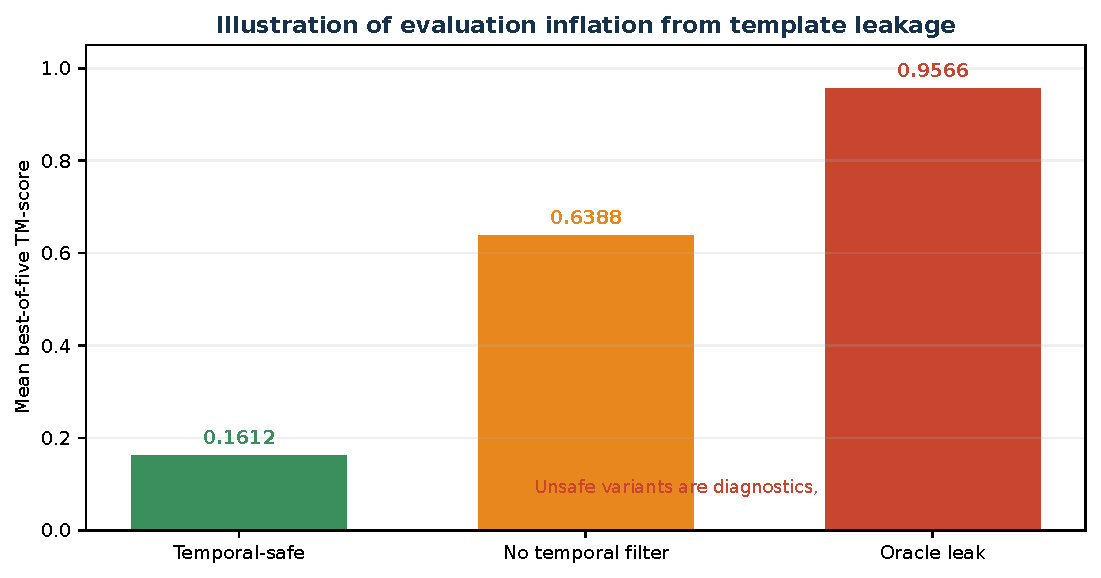
\includegraphics[width=0.77\textwidth]{leakage_diagnostic.pdf}
\caption{Evaluation inflation from template leakage on the development CASP15 cohort.
The unsafe variants are diagnostics only.}
\label{fig:leakage_en}
\end{figure}

\section{Label-use policy}

Native labels are read only by local evaluation scripts after candidate generation.
Within the complementarity analysis, an ``oracle'' is a maximum used to measure the
available ceiling of a candidate bank; it is never an inference-time selector. Geometry
refinement receives only source coordinates, source confidence, and aggregate priors.
For each candidate, the reference conformation used for local metrics is fixed from the
raw candidate so that refinement cannot benefit by switching to an easier native.

The final Kaggle artifact contains no validation labels, hidden labels, or prebuilt
submission. Its manifest records \texttt{native\_labels\_used: false}; the output has
2,515 rows, 18 columns, correct identifiers, and finite coordinates. The final SHA-256 is
\begin{center}
\scriptsize\ttfamily 54fe6e6598a1c2924ef7cbf03482f7ecf3c2e52e8726a1609569f777b1ac8c9a
\end{center}
These checks establish deployment integrity, while Equation~\ref{eq:temporal_gate_en}
governs template validity.

\section{Statistical unit}

The RNA target is the independent unit for every confidence interval. Candidates from
one target share a sequence, native structure, and generation process, and are not
treated as independent observations. For target effects $d_i$, we report
\begin{equation}
\bar d=\frac{1}{n}\sum_{i=1}^{n}d_i
\end{equation}
and a percentile interval from 10,000 bootstrap samples of targets with replacement.
Bootstrap resampling provides a nonparametric estimate of uncertainty from the observed
sample \cite{bootstrap}. The random seed is fixed at 2025.

Effects are oriented so that positive values indicate improvement. TM-score and lDDT
use new minus baseline, whereas RMSD, clash, and deviation use baseline minus new. Tables
also report medians and improve, tie, and regress counts when available, preventing a
mean effect from hiding systematic failures.

\chapter{Proposed Pipeline}
\label{chap:method_en}

\section{Overview}

The pipeline accepts an RNA sequence and temporal cutoff, then generates candidates from
two independent branches. TBM returns three ranked structures, and DRfold2 returns two
structures by internal confidence. When DRfold2 exceeds its resource limit, TBM fills
the unused positions. Geometry refinement processes each candidate independently for
300 steps, and the writer emits exactly five \cprime{} traces.

\begin{figure}[H]
\centering
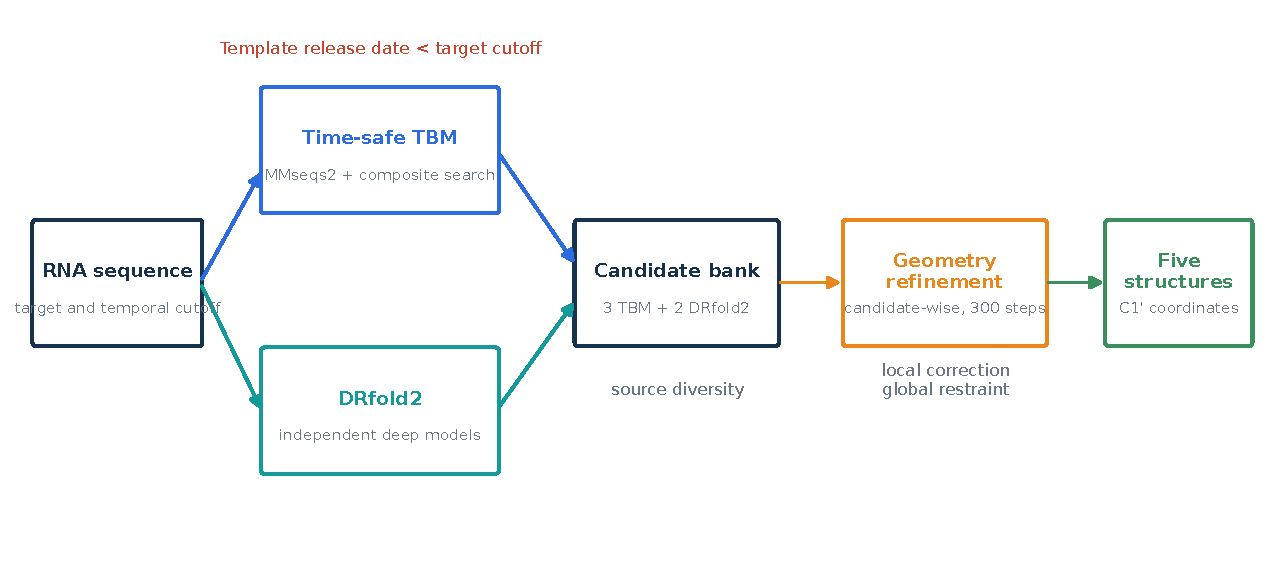
\includegraphics[width=\textwidth]{pipeline_overview.pdf}
\caption{Final pipeline. Source diversity is created before candidate-wise refinement,
with no native-guided selection or coordinate fusion.}
\label{fig:pipeline_en}
\end{figure}

The design follows two principles. First, diversity is introduced at the source level
through three TBM and two DRfold2 candidates. Second, refinement remains close to each
source to avoid disrupting an already correct fold. The two principles address distinct
failure modes and are evaluated separately.

\section{Time-safe TBM}

\subsection{Dual-path retrieval}

The first path runs MMseqs2 over the template-sequence index. MMseqs2 uses accelerated
filters and sensitive alignment to search large collections \cite{mmseqs2}. Raw hits
are normalized to chain keys, identity, alignment coverage, and release dates. Hits that
lack \cprime{} coordinates or violate temporal validity are removed before ranking.

The second path scans the deduplicated library with
\begin{equation}
S_{\mathrm{comp}}(q,s)=0.4G(q,s)+0.3L(q,s)+0.2F(q,s)+0.1K_3(q,s),
\label{eq:composite_en}
\end{equation}
where $G$ is global-alignment similarity, $L$ is local-alignment similarity, $F$ measures
sequence-composition agreement, and $K_3$ is 3-mer overlap. The alignment terms use the
Needleman-Wunsch and Smith-Waterman formulations
\cite{needleman_wunsch,smith_waterman}. The weights are frozen heuristics, and their
sensitivity is tested by ablation rather than assigned a probabilistic interpretation.

\begin{figure}[H]
\centering
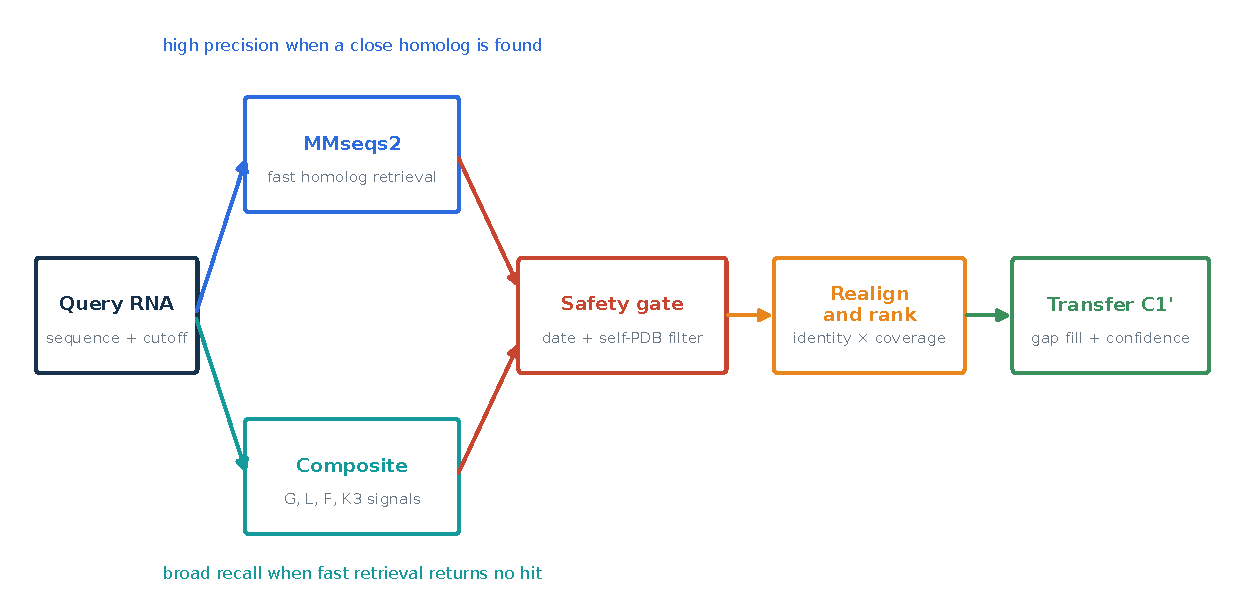
\includegraphics[width=0.98\textwidth]{tbm_flow.pdf}
\caption{TBM flow. MMseqs2 prioritizes clear homologs, composite search broadens recall,
and the safety gate precedes realignment and coordinate transfer.}
\label{fig:tbm_flow_en}
\end{figure}

The two lists are merged by chain key before temporal and self-PDB filtering. The design
in Figure~\ref{fig:tbm_flow_en} keeps the roles separate: MMseqs2 is not considered
inaccurate when no hit is returned, and composite search is not considered accurate
merely because it always returns a candidate. Availability and conditional quality are
reported separately.

\subsection{Realignment and ranking}

Every valid hit is globally realigned to establish one correspondence for transfer. Let
$I$ denote identity on aligned positions, $C_q$ the query fraction with supported
coordinates, and $C_s$ template completeness. The rank score is
\begin{equation}
S_{\mathrm{rank}}=I\,C_q\,C_s.
\label{eq:rank_en}
\end{equation}
Identity times coverage defines the primary order, while completeness breaks cases with
missing coordinates. Distinct PDB sources are preferred where possible, and ablation
tests whether this rule changes oracle TM on the cohort.

The rank score is not a calibrated probability of correctness. It orders candidates
without native access. Multiplication by $C_q$ is especially useful when a high-identity
local hit covers only a small part of the query, as shown by the reranking experiment in
Chapter~\ref{chap:results_en}.

\subsection{Coordinate transfer and gap completion}

For aligned residues, the template \cprime{} coordinate is copied to the corresponding
query position. Unsupported residues receive low confidence. Internal gaps are
interpolated along a curve constrained by neighboring anchors, while terminal regions
are extrapolated from nearby backbone steps. A deterministic de novo trace guarantees
finite output when support is insufficient.

Curved filling makes the candidate valid before refinement; it does not reconstruct a
new motif from native information. The experiment therefore bins gaps by length and
measures SW-RMSD9 only at unsupported residues. Evidence of improvement is confined to
gaps of 9 to 20 nucleotides.

\section{DRfold2 branch}

DRfold2 receives the RNA sequence and predicts structure using a pretrained deep model.
Its publication describes an efficient RNA 3D prediction pipeline developed from DRfold
\cite{drfold,drfold2}. This thesis preserves the pretrained inference path and does not
fine-tune it on the 100 local RNAs. The two candidates with highest model confidence are
converted to the common $L\times3$ \cprime{} representation.

The DRfold2 models are generated independently of TBM hits. Independence here means that
the final branch does not use native quality or TBM scores to alter DRfold2 coordinates;
it does not claim that the pretrained model has no relationship to PDB. Family-disjoint
local splits protect the project cohort from obvious overlap, while the model-training
cutoff remains an external-validity consideration.

The frozen implementation limits DRfold2 to 600 nucleotides. During public execution it
ran on 11 of 12 targets and skipped one 720-nucleotide sequence, which retained five TBM
candidates. The fallback rule was fixed before hidden evaluation.

\section{Geometry refinement}

\subsection{Objective}

Given source candidate $X^{(0)}$, the refinement finds a nearby $X$ that reduces
\begin{equation}
\mathcal{L}(X)=
\lambda_s\mathcal{L}_{\mathrm{source}}+
\lambda_b\mathcal{L}_{\mathrm{backbone}}+
\lambda_a\mathcal{L}_{\mathrm{angle}}+
\lambda_t\mathcal{L}_{\mathrm{torsion}}+
\lambda_c\mathcal{L}_{\mathrm{clash}}+
\lambda_k\mathcal{L}_{\mathrm{kink}}+
\lambda_r\mathcal{L}_{R_g}.
\label{eq:geometry_objective_en}
\end{equation}
Each term addresses a specific failure mode, and the source term limits global drift.
Figure~\ref{fig:refinement_mechanism_en} is a conceptual illustration rather than an
experimental target.

\begin{figure}[H]
\centering
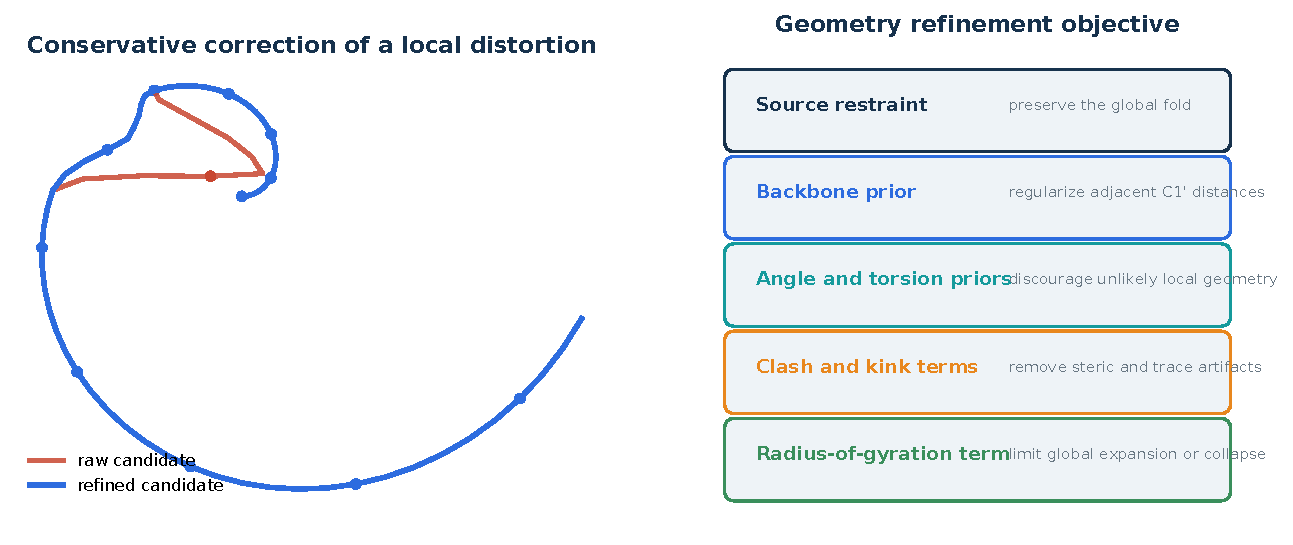
\includegraphics[width=0.98\textwidth]{refinement_mechanism.pdf}
\caption{Geometry refinement mechanism. Local distortion is regularized while a source
restraint preserves the overall arrangement.}
\label{fig:refinement_mechanism_en}
\end{figure}

\subsection{Geometric priors}

Adjacent distance is $d_i=\lVert\mathbf{x}_{i+1}-\mathbf{x}_i\rVert_2$. On the 60 train
RNAs, its mean is 6.09~\angstrom{}, standard deviation is 1.11~\angstrom{}, and median
is 5.66~\angstrom{}. The nonadjacent \cprime{} clash threshold is 4.18~\angstrom{}, and
the radius-of-gyration prior is
\begin{equation}
\widehat R_g(L)=5.18L^{0.346}.
\end{equation}
These values are empirical priors of the frozen project snapshot, not universal physical
constants. They are estimated only on train and held fixed thereafter.

The backbone term uses a context-dependent negative log likelihood of adjacent distance.
Angle and torsion terms operate on consecutive triples and quadruples. Kink and clash
terms penalize sharp bends and close nonadjacent points, while $R_g$ limits global
collapse or expansion. Context-dependent distributions allow more flexibility than one
fixed target distance.

The confidence-weighted source restraint is
\begin{equation}
\mathcal{L}_{\mathrm{source}}=
\frac{1}{L}\sum_{i=1}^{L}w_i
\lVert\mathbf{x}_i-\mathbf{x}^{(0)}_i\rVert_2^2.
\end{equation}
Weights are larger for template-supported or high-confidence residues, allowing gaps and
weak regions to move more than reliable scaffolds. Every candidate is optimized for 300
Adam steps using the configuration frozen on calibration.

\subsection{Baseline and output}

The simple baseline contains only source restraint and backbone smoothing. It tests
whether the additional objective terms improve beyond a conservative local smoother.
The full method is compared with both raw and simple candidates; improvement over raw
alone does not establish the necessity of every term.

After refinement, each candidate is checked for shape, finite values, and residue order.
The writer emits five coordinate triples per nucleotide in exact sample-ID order. The
final pipeline contains no native-guided router, source selection, or coordinate fusion.

\section{Algorithm summary}

\begin{enumerate}
  \item Read sequence $q$, temporal cutoff $t_q$, and excluded PDB identifiers.
  \item Retrieve MMseqs2 and composite hits, then merge by chain key.
  \item Remove hits that violate Equation~\ref{eq:temporal_gate_en}.
  \item Realign, rank, and build three TBM candidates.
  \item Run DRfold2 when $L\leq600$ and retain two candidates by model confidence.
  \item Fill unavailable DRfold2 positions with TBM, maintaining five candidates.
  \item Refine each candidate independently for 300 steps.
  \item Validate identifiers, dimensions, uniqueness, and finite coordinates, then write CSV.
\end{enumerate}

Native labels do not appear in this inference path. All pre-output decisions use sequence,
template metadata, pretrained confidence, and aggregate priors. Oracle scores are
computed only after generation for analysis.

\chapter{Experimental Design}
\label{chap:experiment_en}

\section{Testing strategy}

Each research question is assigned a distinct experiment and maximum claim. RQ1 uses the
20 calibration RNAs to study retrieval sources, composite terms, reranking, and gap
completion. RQ2 uses the 20 validation RNAs to compare candidate banks before refinement.
RQ3 follows the full 60/20/20 protocol and opens validation only after configuration
freeze. This separation prevents exploratory TBM analyses from serving as confirmatory
refinement evidence.

\begin{table}[H]
\centering
\caption{Mapping from research questions to experiments and claims.}
\label{tab:rq_map_en}
\begin{tabularx}{\textwidth}{p{1.0cm}X X}
\toprule
RQ & Primary comparison & Supported claim \\
\midrule
RQ1 & MMseqs2, composite, union; component and reranking ablations & Composite expands availability; ranking effects are measured by component \\
RQ2 & 3T, 2D, union; fixed-N allocation & TBM and DRfold2 complement one another by target \\
RQ3 & Raw, source+backbone, full refinement; cumulative and leave-one-out analyses & Refinement improves local trace within a TM preservation margin \\
\bottomrule
\end{tabularx}
\end{table}

Table~\ref{tab:rq_map_en} constrains interpretation before results are examined. RQ3 does
not hypothesize an increase in TM-score. The validation gate passes when a primary local
metric improves and mean TM change remains within $\pm0.005$, a margin frozen on
calibration.

\section{TBM ablations}

The search-source study compares MMseqs2-only, composite-only, and their union. MMseqs2
TM is conditional on returning a hit, and availability is reported alongside it.
Composite and union means use all 20 targets. This avoids comparing eight easier targets
with a full 20-target cohort as if the samples were equivalent.

The component study compares $G$, $G+L$, $G+L+F$, an equal four-term score, the full
weighted score, and $\pm25\%$ perturbations to individual weights. Useful recall at TM
0.45 is measured within a common candidate pool as an internal diagnostic. An
unsafe-date variant quantifies leakage and is never considered a valid method.

The reranking study begins with identity, then adds query coverage, template completeness,
and distinct-PDB selection. Gap completion compares linear and curved interpolation in
length bins 1-3, 4-8, 9-20, and above 20 nucleotides. Gaps within a target are averaged
before target-level bootstrap.

\section{Complementarity analysis}

Source candidates are evaluated before refinement. For target $i$, let $T_i$ contain the
three TBM scores and $D_i$ the two DRfold2 scores. The source and union ceilings are
\begin{equation}
O_T(i)=\max T_i,\quad O_D(i)=\max D_i,\quad
O_U(i)=\max(T_i\cup D_i).
\end{equation}
The union gain $O_U-O_T$ measures the available value of two additional DRfold2 models.
Because the union has more candidates, it combines source diversity and count effects.

Fixed-N comparisons control this issue. At $N=2$, $2T$ is compared with $1T+1D$; at
$N=3$, $3T$ is compared with $2T+1D$. Candidates are ordered by blind source confidence.
The cache contains only three TBM and two DRfold2 models per target, so a complete
five-slot sweep from $5T$ to $5D$ is not identifiable without duplicating candidates.

\section{Geometry-refinement analysis}

Train estimates priors only. On calibration, cumulative ablation adds source, backbone,
angle, torsion, clash, kink, and $R_g$ terms, while leave-one-out analysis removes each
term from the full objective. The selected configuration satisfies local improvement and
TM preservation, then is serialized before validation.

Validation compares raw candidates, simple source-plus-backbone smoothing, and the full
objective. Primary local metrics are \cprime{}-lDDT, SW-RMSD9, and SW-RMSD15. Best-of-five
TM is the global safeguard, with whole-structure C1 RMSD and SW-RMSD31 as secondary
measures. Backbone deviation, clash, sharp kink, angle NLL, torsion NLL, and $R_g$ error
are mechanism diagnostics because they lie in or near the objective.

A fixed-$N=3$ factorial forms four cells: $3T$ raw, $3T$ refined, $2T+1D$ raw, and
$2T+1D$ refined. It estimates source-bank gain with refinement off, refinement effect
within each bank, and the interaction. This design directly tests whether refinement can
explain the hybrid TM increase.

\section{External evaluation and reproducibility}

Two frozen submissions are compared: time-safe composite TBM and the final hybrid. The
hybrid replaces two TBM positions with DRfold2 when feasible, then applies the frozen
refinement configuration. Public and private scores are read from Kaggle, while the
execution manifest and output hash provide integrity checks \cite{kaggle_competition}.

Repository scripts generate all local tables. Bootstrap seed is 2025, and frozen
configurations, prior provenance, and candidate caches accompany the artifacts. Audits
require one metadata row per target, no cross-split groups, exactly three TBM and two
DRfold2 candidates per target, finite coordinates, and a fixed reference conformation
between raw and refined evaluation.

\chapter{Results}
\label{chap:results_en}

\section{RQ1: TBM retrieval and ranking}

\subsection{Retrieval sources}

MMseqs2 found a template for 8 of 20 calibration RNAs, an availability of 40\%. On those
eight targets, top-1 TM was 0.660029 and best-of-five TM was 0.678316. Composite search
produced candidates for all 20 targets but reached a lower whole-cohort mean of 0.376060.
The union maintained full availability and increased the mean to 0.389705.

\begin{table}[H]
\centering
\caption{Retrieval-source results on 20 calibration RNAs. MMseqs2 quality is conditional
on the eight targets with a hit.}
\label{tab:search_source_en}
\resizebox{\textwidth}{!}{%
\begin{tabular}{lrrr}
\toprule
Source & Targets with hits & Availability & Best-of-five TM when available \\
\midrule
MMseqs2-only & 8/20 & 0.40 & 0.678316 \\
Composite-only & 20/20 & 1.00 & 0.376060 \\
MMseqs2 + composite & 20/20 & 1.00 & 0.389705 \\
\bottomrule
\end{tabular}
}
\end{table}

The sources have distinct roles. MMseqs2 candidates are strong when a homolog is
recognized, while composite search fills the remaining 12 targets at lower average
precision. The union gained 0.013645 over composite-only, although its interval
$[-0.004417,0.042781]$ included zero. The clearest benefit is therefore availability,
not uniform superiority of composite hits.

\subsection{Composite components}

The full weighted score reached 0.376060, whereas global alignment alone reached
0.381177. The G-only advantage was 0.005117 with confidence interval
$[-0.002178,0.015004]$. Perturbing individual weights by $\pm25\%$ produced scores from
0.375436 to 0.376500. The heuristic is locally stable but does not clearly outperform
global alignment on this cohort.

The $G+L+F$ variant nevertheless had useful recall 0.676304 compared with 0.635488 for
G-only within the common hit pool. This pattern is consistent with a recall heuristic:
additional signals introduce distinct candidates even when mean oracle TM does not rise
clearly. Useful recall remains an internal diagnostic rather than a replacement for TM.

Removing the temporal filter increased mean TM from 0.376060 to 0.403022, a change of
0.026962. The interval $[-0.000343,0.071258]$ was wide and 15 targets were unchanged.
This is not evidence for an unsafe method; it shows that a few leaked templates can shift
the cohort mean.

\subsection{Reranking and gap completion}

Adding query coverage to identity increased top-five TM from 0.371900 to 0.387558, a
gain of 0.015659 with interval $[-0.003731,0.045178]$. Completeness and distinct-PDB
selection did not change oracle TM on this cohort, although the latter increased the mean
number of distinct PDB sources. Coverage is therefore the dominant ranking signal in
Table~\ref{tab:tbm_rerank_en}, while later rules primarily support robustness.

\begin{table}[H]
\centering
\caption{TBM reranking ablation.}
\label{tab:tbm_rerank_en}
\begin{tabular}{lrrr}
\toprule
Ranking & Top-1 TM & Top-3 TM & Top-5 TM \\
\midrule
Identity only & 0.334450 & 0.363854 & 0.371900 \\
Identity $\times$ coverage & 0.363720 & 0.378412 & 0.387558 \\
$+\,$template completeness & 0.363720 & 0.378412 & 0.387558 \\
$+\,$distinct PDB & 0.363720 & 0.378412 & 0.387558 \\
\bottomrule
\end{tabular}
\end{table}

Curved gap filling showed clear improvement only for gaps of 9 to 20 nucleotides. It
reduced SW-RMSD9 by 0.036778~\angstrom{} with interval
$[0.009289,0.067605]$. Bins 1-3 and 4-8 showed no clear difference from linear filling,
and gaps above 20 were unchanged. The curve has enough span to avoid a straight bridge
in the middle bin but insufficient information to reconstruct very long missing motifs.

\section{RQ2: Source complementarity}

Before refinement, three TBM candidates reached a mean oracle of 0.565183, and two
DRfold2 candidates reached 0.502627. Their five-candidate union reached 0.588304, a
0.023121 gain over TBM with interval $[0.006444,0.047519]$. DRfold2 supplied the better
source for 8 targets, whereas TBM did so for 12.

\begin{figure}[H]
\centering
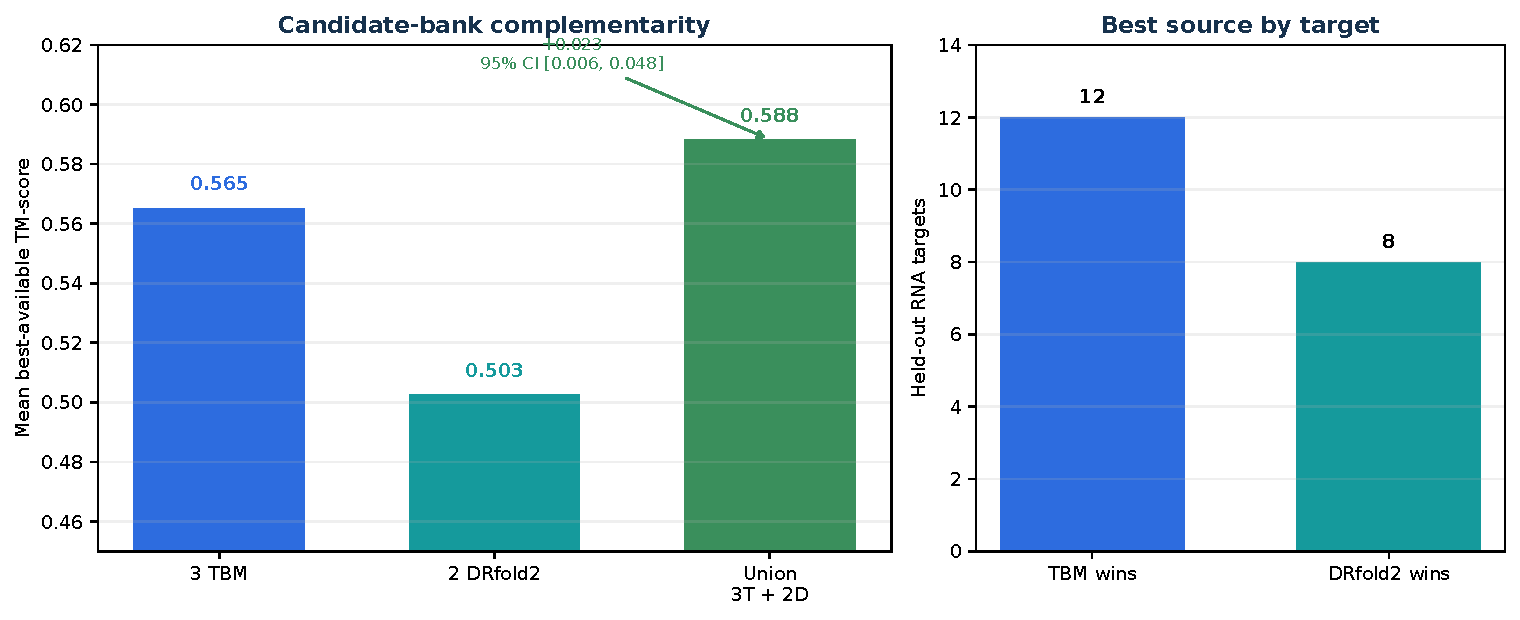
\includegraphics[width=0.92\textwidth]{complementarity_results.pdf}
\caption{Candidate-bank complementarity on 20 validation RNAs. The union interval is
obtained by target-level bootstrap.}
\label{fig:complementarity_en}
\end{figure}

The central result is not higher mean accuracy for DRfold2. Its source mean was 0.062556
below TBM. Its value arose from the eight targets on which source ordering reversed.
Because oracle union cannot decrease when candidates are added, fixed-N comparisons are
required to separate source from count effects.

At two slots, $1T+1D$ exceeded $2T$ by 0.030546 with interval
$[0.002949,0.068185]$. At three slots, $2T+1D$ exceeded $3T$ by 0.016012, although the
interval $[-0.002072,0.041466]$ included zero and ten targets tied. The declining
marginal effect suggests that DRfold2 is most useful when it replaces a redundant
template; three diverse TBM candidates leave less room for improvement.

\begin{table}[H]
\centering
\caption{Candidate allocation with geometry refinement disabled.}
\label{tab:allocation_en}
\resizebox{\textwidth}{!}{%
\begin{tabular}{lrrl}
\toprule
Comparison & Baseline mean & Hybrid mean & Mean gain and 95\% CI \\
\midrule
$2T$ versus $1T+1D$ & 0.549040 & 0.579586 & $+0.030546$ $[0.002949,0.068185]$ \\
$3T$ versus $2T+1D$ & 0.565183 & 0.581196 & $+0.016012$ $[-0.002072,0.041466]$ \\
$3T$ versus $3T+2D$ & 0.565183 & 0.588304 & $+0.023121$ $[0.006444,0.047519]$ \\
\bottomrule
\end{tabular}
}
\end{table}

Table~\ref{tab:allocation_en} distinguishes fixed-size and production-bank effects. In
both the two-slot and three-slot comparisons, replacing one TBM candidate with DRfold2
increased the mean, but only the two-slot confidence interval lay entirely above zero.

\section{RQ3: Geometry refinement}

\subsection{Confirmatory results}

Full refinement increased \cprime{}-lDDT from 0.659836 to 0.666496, a gain of 0.006660
with interval $[0.000933,0.013093]$; 12 of 20 targets improved. SW-RMSD9 decreased from
2.651395 to 2.611010~\angstrom{}, an improvement of 0.040386~\angstrom{} with interval
$[0.029354,0.052090]$ and 19 targets improving. SW-RMSD15 improved by
0.017257~\angstrom{} with interval $[0.000617,0.031336]$.

Global TM changed from 0.588304 to 0.587197, or $-0.001107$ with interval
$[-0.002809,0.000418]$. The effect remained inside the predeclared 0.005 preservation
margin. Whole-structure C1 RMSD and SW-RMSD31 showed no clear change.

\begin{figure}[H]
\centering
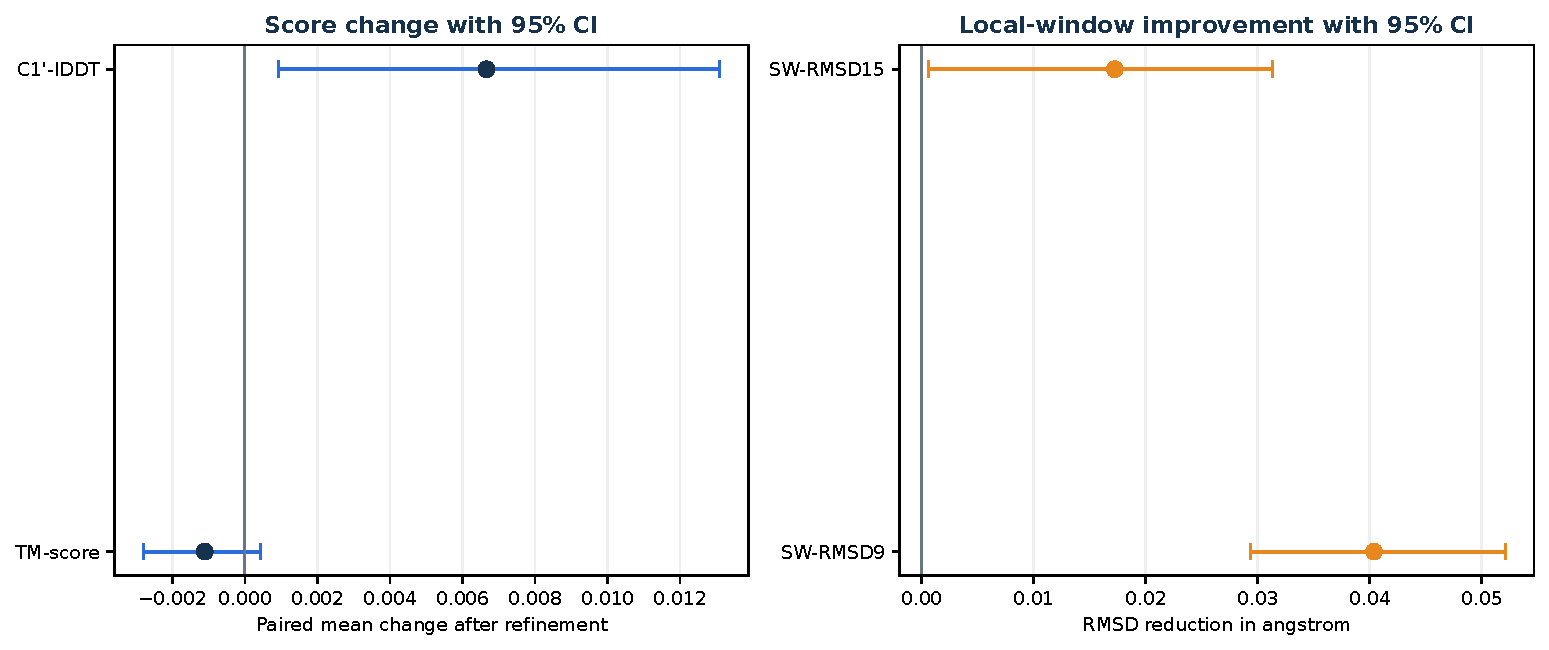
\includegraphics[width=0.94\textwidth]{geometry_results.pdf}
\caption{Confirmatory geometry-refinement effects. Score changes and RMSD reductions use
separate axes and units.}
\label{fig:geometry_results_en}
\end{figure}

\begin{table}[H]
\centering
\caption{Raw and full geometry refinement on 20 validation RNAs.}
\label{tab:geometry_main_en}
\resizebox{\textwidth}{!}{%
\begin{tabular}{lrrrl}
\toprule
Metric & Raw & Refined & Improvement & 95\% CI \\
\midrule
Best-of-five TM & 0.588304 & 0.587197 & $-0.001107$ & $[-0.002809,0.000418]$ \\
\cprime{}-lDDT & 0.659836 & 0.666496 & $+0.006660$ & $[0.000933,0.013093]$ \\
SW-RMSD9 (\angstrom{}) & 2.651395 & 2.611010 & $+0.040386$ & $[0.029354,0.052090]$ \\
SW-RMSD15 (\angstrom{}) & 4.273393 & 4.256136 & $+0.017257$ & $[0.000617,0.031336]$ \\
Backbone deviation (\angstrom{}) & 1.040270 & 0.785817 & $+0.254453$ & diagnostic \\
Clash per residue & 0.065121 & 0.022802 & $+0.042319$ & diagnostic \\
\bottomrule
\end{tabular}
}
\end{table}

The dominant pattern in Table~\ref{tab:geometry_main_en} is stronger improvement at
shorter spatial scales. SW-RMSD9 is the most consistent effect, SW-RMSD15 is smaller,
and SW-RMSD31 and global RMSD are inconclusive. This scale gradient matches the design:
refinement adjusts neighboring relationships rather than rearranging the fold.

\subsection{Simple baseline and ablation}

Source-plus-backbone smoothing increased lDDT by 0.007581, numerically above the full
method's 0.006660. The full-minus-simple difference was $-0.000921$ with interval
$[-0.003118,0.001327]$, so the full objective did not outperform the simple baseline on
lDDT. In contrast, it improved SW-RMSD9 by a further 0.030585~\angstrom{} with interval
$[0.019640,0.044115]$ and corrected angle, torsion, clash, and kink diagnostics that the
simple baseline degraded.

Leave-one-out analysis linked terms to mechanisms. Removing backbone nearly eliminated
the lDDT gain; removing angle or torsion degraded the corresponding NLL; removing kink
increased sharp bends; and removing clash or $R_g$ worsened clash diagnostics. These
results show that the objective behaves as designed, but optimized diagnostics are not
treated as independent evidence. The primary claim remains based on lDDT and
sliding-window RMSD.

\subsection{Source-by-refinement factorial}

Within the $3T$ bank, refinement changed TM by $-0.005852$ with interval
$[-0.014781,0.000724]$. Within $2T+1D$, the effect was $-0.002604$ with interval
$[-0.005473,-0.000278]$. The interaction was $+0.003248$ with an interval containing
zero. Table~\ref{tab:factorial_en} therefore shows a positive source-bank effect before
refinement and no positive TM effect from refinement in either bank.

\begin{table}[H]
\centering
\caption{Fixed-$N=3$ factorial separating source composition and geometry refinement.}
\label{tab:factorial_en}
\begin{tabular}{lrr}
\toprule
Candidate bank & Raw mean TM & Refined mean TM \\
\midrule
$3T+0D$ & 0.565183 & 0.559331 \\
$2T+1D$ & 0.581196 & 0.578592 \\
\bottomrule
\end{tabular}
\end{table}

The factorial contradicts a simple explanation in which refinement causes the hybrid
global-TM gain. Replacing one of three TBM candidates with DRfold2 already produced a
0.016012 mean increase with refinement disabled. Refinement slightly reduced TM in both
banks. Source diversity is therefore the better-supported global mechanism, while
refinement acts on local quality.

\subsection{Subgroups and failure cases}

In a post hoc stratification, initially low-quality candidates gained 0.016261 lDDT with
interval $[0.008900,0.024089]$. High-quality candidates changed by $-0.001788$ with
interval $[-0.005775,0.002420]$. This pattern motivates a future blind quality gate but
cannot revise the current method because the groups were examined after validation.

Three failures remain visible. Targets \texttt{9E2Z\_F} and \texttt{8K7W\_A} lost about
0.009 TM, while \texttt{9B0S\_Et} lost about 0.011 lDDT. Conservative refinement does
not imply monotonic improvement for every target, and both uncertainty and failure
counts are needed beside the mean.

\section{External Kaggle evaluation}

Time-safe composite TBM scored 0.60084 public and 0.60175 private. The final pipeline
reached 0.62809 and 0.61390, absolute gains of 0.02725 and 0.01215. The reference
TBM-only notebook reported 0.59298 private \cite{kaggle_top1}; the final pipeline was
0.02092 higher.

\begin{figure}[H]
\centering
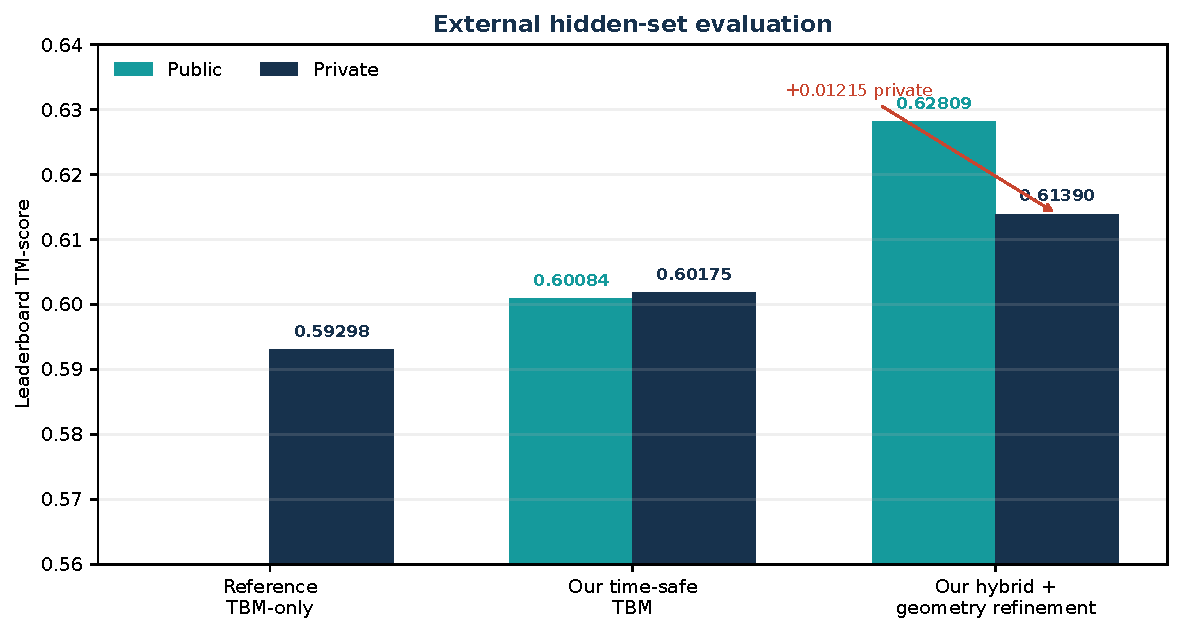
\includegraphics[width=0.86\textwidth]{leaderboard_results.pdf}
\caption{Hidden-set evaluation. Only a private score is reported for the reference
notebook; both public and private scores are available for the thesis pipelines.}
\label{fig:leaderboard_en}
\end{figure}

The public execution provides deployment checks. DRfold2 generated two candidates for
11 of 12 targets, the 720-nucleotide target used five TBM candidates, and refinement
completed for all 60 structures. Output shape and identifiers were valid, and the run
did not read native labels. These observations support execution integrity but cannot
identify which hidden targets produced the score increase.

The Kaggle result must be read with the local factorial. The final submission both
replaced two TBM slots and applied refinement, making the private change a pipeline-level
effect. Local evidence shows that hybrid composition improves global TM before
refinement, whereas refinement improves local metrics and slightly reduces TM. Together,
the two evidence levels explain the higher score without attributing it wholesale to
geometry refinement.

\begin{figure}[H]
\centering
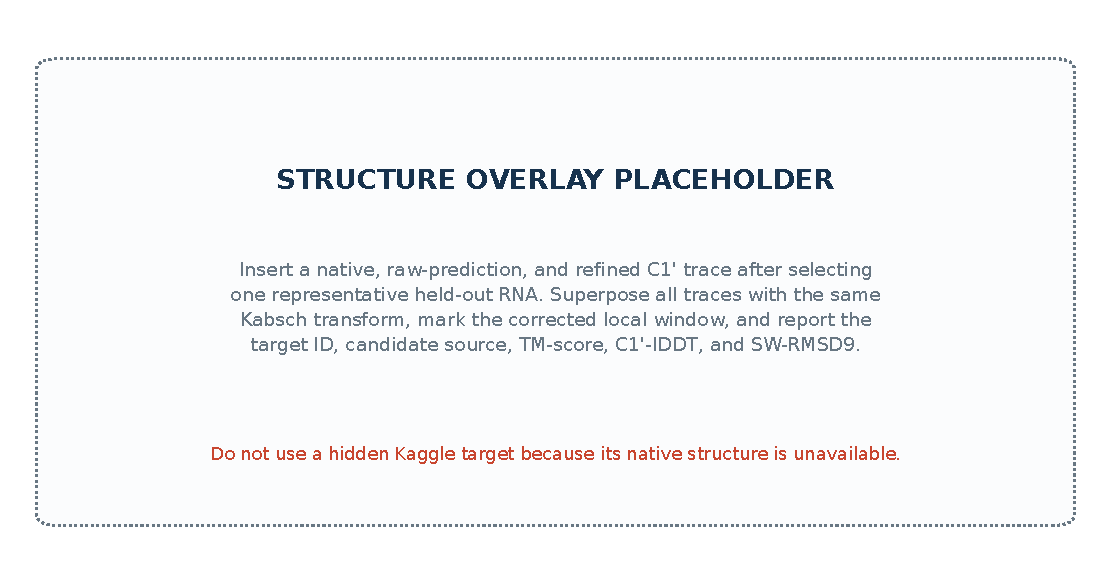
\includegraphics[width=0.88\textwidth]{structure_overlay_placeholder.pdf}
\caption{Controlled placeholder for a native, raw, and refined structure overlay. The
final figure should use a public validation RNA with complete provenance, never a hidden
Kaggle target.}
\label{fig:overlay_placeholder_en}
\end{figure}

Figure~\ref{fig:overlay_placeholder_en} is intentionally a placeholder rather than a
fabricated example. A representative target should be selected by a declared rule, such
as SW-RMSD9 change nearest the median. The final caption should record target identifier,
candidate source, raw and refined metrics, highlighted window, and generation script.

\chapter{Discussion}
\label{chap:discussion_en}

\section{Why the hybrid pipeline has value}

The gain over the TBM-only reference does not require one source to dominate everywhere.
TBM had the higher source mean and won on 12 targets, while DRfold2 won on the remaining
eight. Under best-of-five scoring, a distinct source only needs to win a substantial
subset of targets to improve the union mean. Complementarity is therefore a target-wise
property rather than a comparison of source averages.

The two-slot fixed-N result strengthens this argument by removing candidate-count
advantage. Replacing one of two TBM structures with a DRfold2 structure retained a
positive confidence interval. The three-slot effect was weaker because three TBM models
already contained more diversity and the validation cohort contained only 20 targets.
The three-plus-two allocation is consequently a reasonable compromise for the hidden
distribution, not a universal optimum.

Competition data provide a second explanation. The analysis reported that 19 of 20
private targets had a prior structure with TM-align above 0.45, a higher template-rich
fraction than CASP15 \cite{competition_paper}. A large template snapshot and broad
retrieval were advantageous in this regime. The same paper cautions that this ordering
may not generalize to template-poor RNA \cite{competition_paper}; DRfold2 remains an
important hedge against that part of the distribution.

\section{Why refinement does not increase TM-score}

The source restraint places the optimum near the starting candidate. Backbone, angle,
torsion, and clash terms operate mainly on short-range relationships and contain no
signal for changing topology or moving an entire domain. Improvement in lDDT and
SW-RMSD9 with nearly unchanged TM is therefore consistent with the intended mechanism.

An incorrect global fold requires long-range contacts, motif information, or a different
template. Local optimization around one source cannot invent this evidence. Nucleic-acid
refinement studies likewise distinguish improved stereochemistry from systematic native
RMSD improvement \cite{qrnas}. Geometry refinement should therefore be interpreted as
trace regularization, with source diversity setting the primary global ceiling.

The simple baseline matched the full method on lDDT, identifying backbone smoothing as
the principal mechanism for that score. The full objective showed clearer value for
SW-RMSD9 and balanced angle, torsion, clash, and kink diagnostics. This narrows the
contribution: the full objective is not necessary for every local gain, but it provides
a more balanced trace without disrupting the average fold.

\section{Interpreting the leaderboard}

The 0.61390 private score has value because it is measured on hidden structures and
exceeds both the project's TBM pipeline and the reference notebook. It establishes that
the complete implementation transfers beyond the local cohort. A scalar score, however,
does not reveal the per-target counterfactual obtained by disabling one component.

A defensible explanation therefore has three layers. The integrity audit shows that the
submission does not use native labels and enforces temporal filtering. The local
complementarity analysis identifies a positive global mechanism. The local refinement
analysis identifies a separate local mechanism and shows that it does not increase TM.
Together, these layers explain performance while preserving the distinction between
external validity and component causality.

Distribution shift is also visible. The frozen hybrid rule scored 0.46450 on the 12
CASP15 targets and was worse than the local TBM bank, whereas it improved Kaggle private
TM by 0.01215. This reversal shows that effective allocation depends on the target
distribution. Reporting both outcomes is more credible than selecting the favorable
cohort and argues against a universally optimal mixture.

\section{Threats to validity}

\subsection{Internal validity}

Calibration and validation contain only 20 targets each, leaving wide intervals for
several ablations. Target bootstrap handles dependence among candidates but cannot create
information beyond the observed RNAs \cite{bootstrap}. Multiple subgroup analyses also
increase the chance of incidental patterns, so they are labeled post hoc and do not
change the current method.

The cache contains only three TBM and two DRfold2 candidates. Fixed-N comparisons up to
three positions are identified, but a full five-position allocation sweep is not. Future
work should generate at least five independent candidates from each source before
opening a new cohort.

\subsection{External validity}

Local validation covers single-chain RNA up to 96 nucleotides. Refinement results do not
directly generalize to 720-nucleotide RNA, multichain complexes, or RNA-protein interfaces.
Such systems have different interaction patterns and experimental uncertainties
\cite{zhang_experimental_review,ma_cryoem}.

The Kaggle private set is unusually template rich \cite{competition_paper}. Its score
supports the competition distribution but does not guarantee the same ordering on a
template-poor benchmark. A new temporal benchmark released after 2026 would provide a
stronger generalization test.

\subsection{Metric validity}

TM-score and \cprime{}-lDDT evaluate a coarse-grained trace. They do not directly measure
base orientation, hydrogen bonding, ion coordination, or full-atom stereochemistry,
all of which contribute to tertiary interactions and RNA function
\cite{butcher_tertiary,cao_rna_functions}. A high-scoring trace is therefore not yet a
complete model for docking or mechanistic interpretation.

Angle NLL, torsion NLL, clash, and kink are objective diagnostics and favor the full
method by construction. They explain mechanism but cannot replace independent metrics.
Prioritizing lDDT, sliding-window RMSD, and TM reduces circularity, while full-atom
validation remains necessary for biochemical use.

\section{Future work}

The nearest extension is quality-gated refinement. Post hoc results suggest larger lDDT
gains for weak candidates than strong ones. A blind gate could skip refinement when
source confidence and self-consistency are high, but it must be preregistered on a new
calibration set and tested on an unopened cohort.

A second direction is greater within-source diversity. Five independent TBM and five
DRfold2 models would support a complete allocation sweep and measure the marginal return
of each position. A third direction is full-atom reconstruction with an evaluated tool
such as Arena, followed by stereochemical metrics designed for RNA
\cite{arena,rna_puzzles_toolkit}.

Finally, temporal metadata should fail closed, and self-PDB exclusion should parse target
reference identifiers directly. These changes improve auditability rather than score. In
a field with continuously released structural data, reconstructing what was known at
prediction time is essential to meaningful evaluation.

\chapter{Conclusion}
\label{chap:conclusion_en}

This thesis developed and evaluated an RNA 3D pipeline composed of time-safe TBM,
DRfold2, and geometry refinement. Rather than treating the final score as the only
evidence, the study separated retrieval, source diversity, and local postprocessing into
three questions with distinct ablations and protocols.

For RQ1, MMseqs2 produced strong candidates when a homolog was found but covered only 8
of 20 calibration RNAs. Composite search expanded availability to all 20 targets. The
full weighted score did not clearly beat global alignment alone, and query coverage was
the most influential reranking component. Composite search is therefore supported as a
recall heuristic within time-safe TBM.

For RQ2, TBM had higher average source quality, but TBM and DRfold2 won on different
targets. Their union improved mean best-available TM by 0.023121 with a positive
confidence interval, and the fixed-$N=2$ comparison retained a 0.030546 gain. These
results directly show that source diversity can improve best-of-five performance without
one source universally outperforming the other.

For RQ3, geometry refinement increased \cprime{}-lDDT by 0.006660, reduced SW-RMSD9 by
0.040386~\angstrom{}, and changed TM by $-0.001107$. A simple smoother explained much
of the lDDT gain, while the full objective improved short-window RMSD and geometric
diagnostics. The supported conclusion is local trace correction with average global-fold
preservation.

The final pipeline reached 0.62809 public and 0.61390 private, exceeding the project TBM
pipeline and the reference TBM-only score. The local factorial identifies candidate
complementarity as the better-supported mechanism for global improvement, while geometry
refinement provides a separate local benefit. This distinction is the thesis's central
scientific value: it reports a competitive system while stating precisely which evidence
supports each mechanism and where that evidence ends.

\appendix

\chapter{Reproducibility Artifacts}
\label{app:repro_en}

The principal artifacts are:
\begin{itemize}
  \item \path{scripts/run_tbm_whitebox_ablation.py} for the TBM component study;
  \item \path{scripts/summarize_hybrid_complementarity.py} for source allocation;
  \item \path{reports/thesis_notes/tbm_whitebox_ablation.md} for RQ1 tables;
  \item \path{reports/thesis_notes/hybrid_complementarity.md} for RQ2 tables;
  \item \path{reports/thesis_notes/kaggle_submission_analysis.md} for external scores and manifests;
  \item \path{scripts/generate_thesis_v2_figures.py} for all data figures in this draft.
\end{itemize}

The confirmatory runner, its detailed RQ3 report, and the frozen configuration remain in
the repository. The final release should add a manifest with the Git commit, Python
environment, template-database checksum, pretrained-model version, and exact command for
every table.

\chapter{Figure Completion Checklist}

Figure~\ref{fig:overlay_placeholder_en} is the only intentional placeholder. To complete
it, select one validation target by a fixed criterion; read its public native structure,
raw candidate, and refined candidate; apply one correspondence and Kabsch convention;
plot the three traces with consistent residue indices; mark a representative local
window; and record source paths and metrics in the caption.

All other figures are generated from frozen aggregates by the script listed in
Appendix~\ref{app:repro_en}. Before submission, check fonts, grayscale contrast, text size
at 100\%, and every plotted number against its source table.

\begin{thebibliography}{99}

\bibitem{zhang_experimental_review}
J. Zhang, Y. Fei, L. Sun, and Q. C. Zhang,
``Advances and opportunities in RNA structure experimental determination and computational modeling,''
\emph{Nature Methods}, vol. 19, pp. 1193-1207, 2022.
doi: 10.1038/s41592-022-01623-y.

\bibitem{cao_rna_functions}
X. Cao, Y. Zhang, Y. Ding, and Y. Wan,
``Identification of RNA structures and their roles in RNA functions,''
\emph{Nature Reviews Molecular Cell Biology}, vol. 25, pp. 784-801, 2024.
doi: 10.1038/s41580-024-00748-6.

\bibitem{tinoco_folding}
I. Tinoco Jr. and C. Bustamante,
``How RNA folds,''
\emph{Journal of Molecular Biology}, vol. 293, no. 2, pp. 271-281, 1999.
doi: 10.1006/jmbi.1999.3001.

\bibitem{butcher_tertiary}
S. E. Butcher and A. M. Pyle,
``The Molecular Interactions That Stabilize RNA Tertiary Structure: RNA Motifs, Patterns, and Networks,''
\emph{Accounts of Chemical Research}, vol. 44, no. 12, pp. 1302-1311, 2011.
doi: 10.1021/ar200098t.

\bibitem{ma_cryoem}
H. Ma, X. Jia, K. Zhang, and Z. Su,
``Cryo-EM advances in RNA structure determination,''
\emph{Signal Transduction and Targeted Therapy}, vol. 7, article 58, 2022.
doi: 10.1038/s41392-022-00916-0.

\bibitem{pdb_archive}
S. K. Burley and coauthors,
``Protein Data Bank: the single global archive for 3D macromolecular structure data,''
\emph{Nucleic Acids Research}, vol. 47, no. D1, pp. D520-D528, 2019.
doi: 10.1093/nar/gky949.

\bibitem{rna_puzzles}
J. A. Cruz and coauthors,
``RNA-Puzzles: A CASP-like evaluation of RNA three-dimensional structure prediction,''
\emph{RNA}, vol. 18, no. 4, pp. 610-625, 2012.
doi: 10.1261/rna.031054.111.

\bibitem{rna_puzzles_toolkit}
M. Magnus, M. Antczak, T. Zok, and coauthors,
``RNA-Puzzles toolkit: a computational resource of RNA 3D structure benchmark datasets, structure manipulation, and evaluation tools,''
\emph{Nucleic Acids Research}, vol. 48, no. 2, pp. 576-588, 2020.
doi: 10.1093/nar/gkz1108.

\bibitem{casp15}
R. Das and coauthors,
``Assessment of three-dimensional RNA structure prediction in CASP15,''
\emph{Proteins: Structure, Function, and Bioinformatics}, vol. 91, no. 12, pp. 1747-1770, 2023.
doi: 10.1002/prot.26602.

\bibitem{state_of_rnart}
C. Bernard, G. Postic, S. Ghannay, and F. Tahi,
``State-of-the-RNArt: benchmarking current methods for RNA 3D structure prediction,''
\emph{NAR Genomics and Bioinformatics}, vol. 6, no. 2, article lqae048, 2024.
doi: 10.1093/nargab/lqae048.

\bibitem{rna_progress_review}
X. Wang, S. Yu, E. Lou, Y. L. Tan, and Z. J. Tan,
``RNA 3D Structure Prediction: Progress and Perspective,''
\emph{Molecules}, vol. 28, no. 14, article 5532, 2023.
doi: 10.3390/molecules28145532.

\bibitem{competition_paper}
Y. Lee, S. He, T. Oda, and coauthors,
``Template-based RNA structure prediction advanced through a blind code competition,''
\emph{bioRxiv}, preprint 2025.12.30.696949, 2025.
doi: 10.64898/2025.12.30.696949.

\bibitem{mmseqs2}
M. Steinegger and J. S\"oding,
``MMseqs2 enables sensitive protein sequence searching for the analysis of massive data sets,''
\emph{Nature Biotechnology}, vol. 35, pp. 1026-1028, 2017.
doi: 10.1038/nbt.3988.

\bibitem{needleman_wunsch}
S. B. Needleman and C. D. Wunsch,
``A general method applicable to the search for similarities in the amino acid sequence of two proteins,''
\emph{Journal of Molecular Biology}, vol. 48, no. 3, pp. 443-453, 1970.
doi: 10.1016/0022-2836(70)90057-4.

\bibitem{smith_waterman}
T. F. Smith and M. S. Waterman,
``Identification of common molecular subsequences,''
\emph{Journal of Molecular Biology}, vol. 147, no. 1, pp. 195-197, 1981.
doi: 10.1016/0022-2836(81)90087-5.

\bibitem{drfold}
Y. Li, C. Zhang, C. Feng, R. Pearce, P. L. Freddolino, and Y. Zhang,
``Integrating end-to-end learning with deep geometrical potentials for ab initio RNA structure prediction,''
\emph{Nature Communications}, vol. 14, article 5745, 2023.
doi: 10.1038/s41467-023-41303-9.

\bibitem{rhofoldplus}
T. Shen, Z. Hu, S. Sun, and coauthors,
``Accurate RNA 3D structure prediction using a language model-based deep learning approach,''
\emph{Nature Methods}, vol. 21, pp. 2287-2298, 2024.
doi: 10.1038/s41592-024-02487-0.

\bibitem{drfold2}
Y. Li, C. Feng, X. Zhang, S. Tsukiyama, D. Feng, and Y. Zhang,
``DRfold2 is a deep learning-based tool that enables efficient and accurate RNA structure prediction,''
\emph{PLOS Biology}, vol. 24, no. 2, article e3003659, 2026.
doi: 10.1371/journal.pbio.3003659.

\bibitem{ares}
R. J. L. Townshend, S. Eismann, A. M. Watkins, and coauthors,
``Geometric deep learning of RNA structure,''
\emph{Science}, vol. 373, no. 6558, pp. 1047-1051, 2021.
doi: 10.1126/science.abe5650.

\bibitem{qrnas}
P. Stasiewicz, S. Mukherjee, C. Nithin, and J. M. Bujnicki,
``QRNAS: software tool for refinement of nucleic acid structures,''
\emph{BMC Structural Biology}, vol. 19, article 5, 2019.
doi: 10.1186/s12900-019-0103-1.

\bibitem{arena}
Z. R. Perry, A. M. Pyle, and C. Zhang,
``Arena: Rapid and Accurate Reconstruction of Full Atomic RNA Structures From Coarse-grained Models,''
\emph{Journal of Molecular Biology}, vol. 435, article 168210, 2023.
doi: 10.1016/j.jmb.2023.168210.

\bibitem{tm_score}
Y. Zhang and J. Skolnick,
``Scoring function for automated assessment of protein structure template quality,''
\emph{Proteins: Structure, Function, and Bioinformatics}, vol. 57, no. 4, pp. 702-710, 2004.
doi: 10.1002/prot.20264.

\bibitem{usalign}
C. Zhang, M. Shine, A. M. Pyle, and Y. Zhang,
``US-align: universal structure alignments of proteins, nucleic acids, and macromolecular complexes,''
\emph{Nature Methods}, vol. 19, pp. 1109-1115, 2022.
doi: 10.1038/s41592-022-01585-1.

\bibitem{lddt}
V. Mariani, M. Biasini, A. Barbato, and T. Schwede,
``lDDT: a local superposition-free score for comparing protein structures and models using distance difference tests,''
\emph{Bioinformatics}, vol. 29, no. 21, pp. 2722-2728, 2013.
doi: 10.1093/bioinformatics/btt473.

\bibitem{kabsch}
W. Kabsch,
``A solution for the best rotation to relate two sets of vectors,''
\emph{Acta Crystallographica Section A}, vol. 32, pp. 922-923, 1976.
doi: 10.1107/S0567739476001873.

\bibitem{bootstrap}
B. Efron and R. J. Tibshirani,
\emph{An Introduction to the Bootstrap}.
New York, NY, USA: Chapman and Hall/CRC, 1993.

\bibitem{kaggle_competition}
Stanford University and Kaggle,
``Stanford RNA 3D Folding,''
Kaggle competition documentation, 2025.
Available: \url{https://www.kaggle.com/competitions/stanford-rna-3d-folding}.

\bibitem{kaggle_top1}
JaeJohn,
``RNA 3D folds - TBM only approach,''
Kaggle notebook, version 1, 2025.
Available: \url{https://www.kaggle.com/code/jaejohn/rna-3d-folds-tbm-only-approach}.

\end{thebibliography}


\end{document}
